%note on pictures

% ellipsoid_ridges 
% ./blind -f data/ellipsoid_u_0.02.off -d4 -m4 -a3 -t3 
% ../../demo/Ridges_3/introspect-qt data/ellipsoid_u_0.02.off data/data_ellipsoid_u_0.02.offRIDGES-d4-m4-t3-a3-p0.4ogl.txt 0 0

%david pict for old algo, don't know parameters, todo... and get better pict

%\newcommand{\makeremark}[2]{{
%  \newcommand{#1}[1]
%    {$\longrightarrow$\textsc{#2: ##1}$\leftarrow$\\}}}
%\makeremark{\FC}{Fr\'ed\'eric says}

\newcommand{\FC}[1]{\protect{===FC SAYS: {#1}}}



\newtheorem{definition}{Definition.}
\newcommand{\hot}{h.o.t}%[0]


\begin{figure}[!ht]
\begin{ccTexOnly}
\centerline{
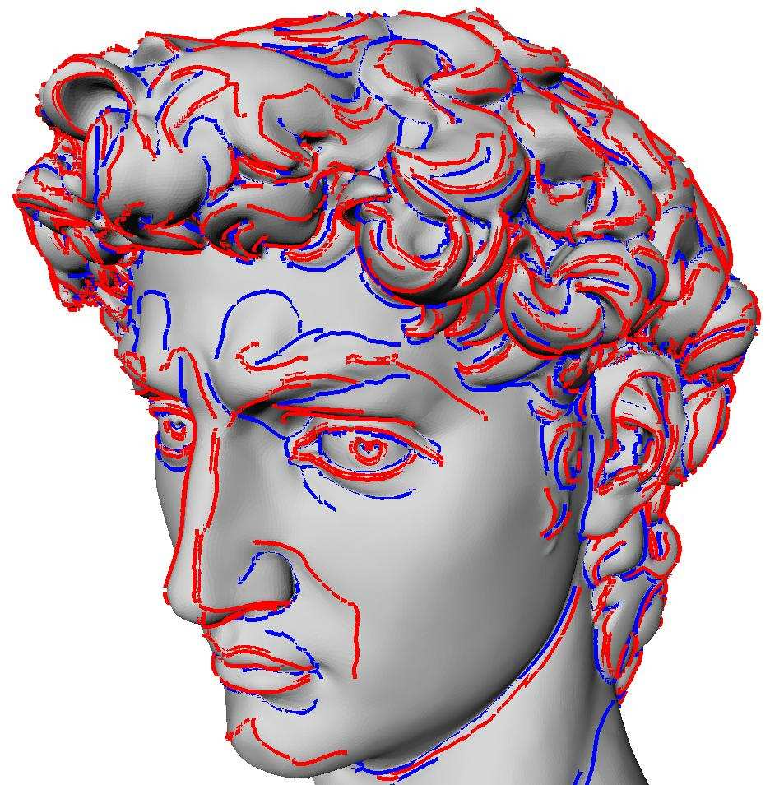
\includegraphics[width=.5\linewidth]{Ridges_3/david_crest}}
\end{ccTexOnly}
\caption{Crest ridges on the David.}
\label{david_crest}
\begin{ccHtmlOnly}
<CENTER> <img border=0 src="./david_crest.png" width=400>
</CENTER>
\end{ccHtmlOnly}
\end{figure}

This chapter describes the \cgal's package for the extraction of
ridges and umbilics on meshes.  Given a smooth surface, a ridge is a
curve along which one of the principal curvatures has an extremum
along its curvature line. An umbilic is a point at which both
principal curvatures are equal. Umbilics are special points on the
ridge lines. Ridges are curves of {\em extremal} curvature and
therefore encode important informations used in segmentation,
registration, matching and surface analysis.  Based on the results of
the article \cite{cgal:cp-tdare-05}, we propose algorithms to identify
and extract different parts of this singular ridge curve as well as
umbilics on a surface given as a triangular mesh. Differential
quantities associated to the mesh vertices are assumed to be given for
these algorithms; such quantities may be computed by the package {\em
Estimation of Local Differential Properties of Sampled Surfaces via
Polynomial Fitting}.


\subsection{Overview}
%%%%%%%%%%%%%%%%%%%%%%

Section \ref{smooth} presents the basics of the theory of ridges and
umbilics on smooth surfaces. Sections \ref{ridge-mesh} and
\ref{umbilic-mesh} present algorithms for the extracting ridges and
umbilics on triangular meshes. Section
\ref{soft} gives the package specifications, while example calls to
functions of the package are provided in section \ref{examples}.


\section{Ridges and umbilics of a smooth surface}
\label{smooth}
%%%%%%%%%%%%%%%%%%%%%%%%%%%%%%%%%%%%%%%

\FC{I did not find cp-ssulc-05 in cgal_manual.bib???????}

For a detailed introduction to ridges and related topics, the reader
may consult 
\cite{cgal:hgygm-ttdpf-99,cgal:p-gd-01}, as well as
the following survey article \cite{cgal:cp-dtges-05}.
%%
In the sequel, we just introduce the basic notions so as to explain
our algorithms.  Consider a smooth embedded surface, and denote $k_1$
and $k_2$ the principal curvatures, with $k_1\geq k_2$. Umbilics are
the points where $k_1=k_2$.  For any non umbilical point, the
corresponding principal directions of curvature are well defined, and
we denote them $d_1$ and $d_2$.
%%
Anything related to the maximal (minimal) curvature is qualified blue
(red), for example we shall speak of the blue curvature for $k_1$ or
the red direction for $d_2$.
%%
In local coordinates, we denote $\langle , \rangle$ the inner product
induced by the ambient Euclidean space, and $dk_1$, $dk_2$ the
gradients of the principal curvatures. Ridges, illustrated on figure
\ref{ellipsoid_ridges}, are defined by:

\begin{definition}
\label{def:ridge-extrema}
A non umbilical point is called
\begin{itemize}
\item
a blue ridge point if the {\em extremality coefficient} $b_0=\langle
dk_1,d_1 \rangle$ vanishes, i.e. $b_0=0$.

\item
a red ridge point if the {\em extremality coefficient} $b_3=\langle
dk_2,d_2 \rangle$ vanishes, i.e. $b_3=0$.

\end{itemize}
\end{definition}

%%
The previous characterization of ridges involves third-order
differential properties. Using fourth-order differential quantities, a
ridge point can further be qualified as {\em elliptic} if it
corresponds to a maximum of $k_1$ or a minimum of $k_2$, or {\em
hyperbolic} otherwise. Hence we end with four types of ridges, namely
: \ccc{BLUE_ELLIPTIC_RIDGE}, \ccc{BLUE_HYPERBOLIC_RIDGE}, \ccc{RED_ELLIPTIC_RIDGE},
\ccc{RED_HYPERBOLIC_RIDGE}, see figure \ref{ellipsoid_ridges}.
In addition, a subset of elliptic ridges, called the crest lines,
which can be seen as the visually most salient curves on a surface are
also of interest. A crest line is an elliptic ridge which is a maximum
of $\max(|k_1|,|k_2|)$. Hence we provide two additional ridge types :
\ccc{BLUE_CREST_RIDGE} and \ccc{RED_CREST_RIDGE}, see figure \ref{david_crest}.


\begin{figure}[!ht]
\begin{ccTexOnly}
\centerline{
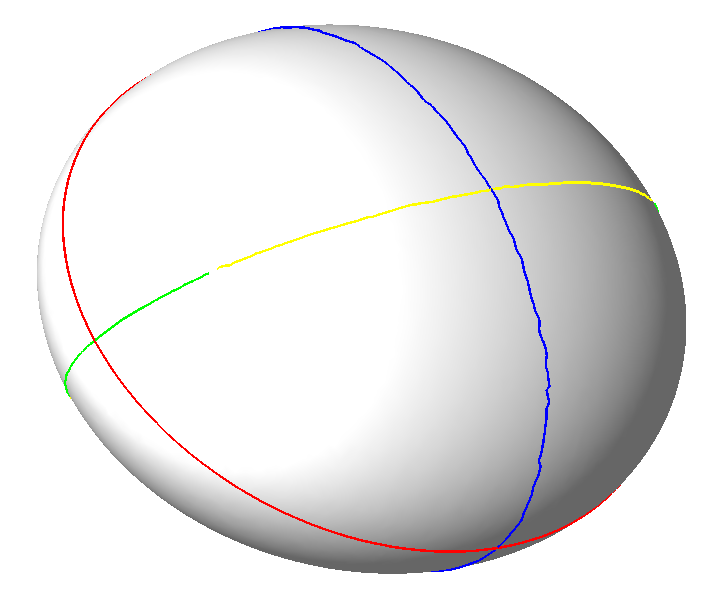
\includegraphics[width=.5\linewidth]{Ridges_3/ellipsoid_ridges}}
\end{ccTexOnly}
\caption{Ridges on the ellipsoid, normals pointing outward.
 Color coding~: \ccc{BLUE_ELLIPTIC_RIDGE} are blue,
\ccc{BLUE_HYPERBOLIC_RIDGE} are green, \ccc{RED_ELLIPTIC_RIDGE} are red and 
\ccc{RED_HYPERBOLIC_RIDGE} are yellow.}
\label{ellipsoid_ridges}
\begin{ccHtmlOnly}
<CENTER> <img border=0 src="./ellipsoid_ridges.png" width=400>
</CENTER>
\end{ccHtmlOnly}
\end{figure}

At any point of the surface which is not an umbilic, principal
directions $d_1, d_2$ are well defined, and these (non oriented)
directions together with the normal vector $n$ define two direct
orthonormal frames. If $v_1$ is a unit vector of direction $d_1$ then
there exists a unique unit vector $v_2$ so that $(v_1,v_2,n)$ is
direct (and the other possible frame is $(-v_1,-v_2,n)$). In the
coordinate systems $(v_1,v_2,n)$, the surface has the following
canonical form, known as the Monge form~:
%
\begin{eqnarray}
\label{eq:monge}
z(x,y) =  & \frac{1}{2}(k_1x^2 + k_2y^2)+
	\frac{1}{6}(b_0x^3+3b_1x^2y+3b_2xy^2+b_3y^3) \\
  &  +\frac{1}{24}(c_0x^4+4c_1x^3y+6c_2x^2y^2+4c_3xy^3+c_4y^4) + \hot
\end{eqnarray}

\noindent The Taylor expansion of $k_1$ (resp. $k_2$) along the blue
(resp. red) curvature line going through the origin and parameterized
by $x$ (resp. $y$) are:
\begin{equation}
\label{eq:taylor_along_line}
k_1(x) = k_1 + b_0x + \frac{P_1}{2(k_1-k_2)}x^2 +\hot \quad \quad \quad,
P_1= 3b_1^2+(k_1-k_2)(c_0-3k_1^3).
\end{equation}
%
\begin{equation}
\label{eq:taylor_along_red_line}
k_2(y) = k_2 + b_3y + \frac{P_2}{2(k_2-k_1)}y^2 +\hot \quad \quad \quad,
P_2= 3b_2^2+(k_2-k_1)(c_4-3k_2^3).
\end{equation}

\noindent Notice also that switching from one to the other of the two
afore-mentioned coordinate systems reverts the sign of all the odd
coefficients on the Monge form of the surface.
\medskip

Hence ridge types are characterized by 
\begin{itemize}
\item
\ccc{BLUE_RIDGE} if $b_0=0$
\item
\ccc{BLUE_ELLIPTIC_RIDGE} if  $b_0=0$ and $P_1<0$
\item
 \ccc{BLUE_HYPERBOLIC_RIDGE} if  $b_0=0$ and $P_1>0$
\item
 \ccc{RED_RIDGE} if  $b_3=0$
\item
 \ccc{RED_ELLIPTIC_RIDGE} if  $b_3=0$ and $P_2<0$
\item
\ccc{RED_HYPERBOLIC_RIDGE} if  $b_3=0$ and $P_2>0$
\item
\ccc{BLUE_CREST_RIDGE} if  $b_0=0$  and $P_1<0$ and $|k_1|>|k_2|$
\item
\ccc{RED_CREST_RIDGE} if  $b_3=0$ and $P_2<0$ and $|k_2|>|k_1|$
\end{itemize}

\FC{picture for the index}
\FC{I removed  $k_1=k_2$ as umbilics have been defined several times before}


As illustrated on Fig. \ref{umbilics} and \ref{}, the patterns made by
curvature lines around an umbilic can be characterized using the
notion of {\em index} associated to the principal directions ---see
also \cite{cgal:cp-dtges-05}.
%%
As depicted on Fig. \ref{}, consider a small circuit $C$ around the
umbilic, and a point $p \in C$. Starting from an initial orientation
$u$ of a tangent vector to the curvature line through point $p$,
propagate {\em by continuity} this orientation around the circuit.  The
index is defined by the angle swept by $u$ around this revolution,
normalized by $2\pi$. On our example, the index is thus ???????.

If the index of the principal direction field is $1/2$
then it is called a
\ccc{UMBILIC_WEDGE}, if it is $-1/2$ it is called a \ccc{UMBILIC_TRISECTOR}.
 Otherwise the umbilic is qualified
\ccc{UMBILIC_NON_GENERIC}.

\FC{find the right figure: asymptotes are missing}

\begin{figure}[!ht]
\begin{ccTexOnly}
\centerline{
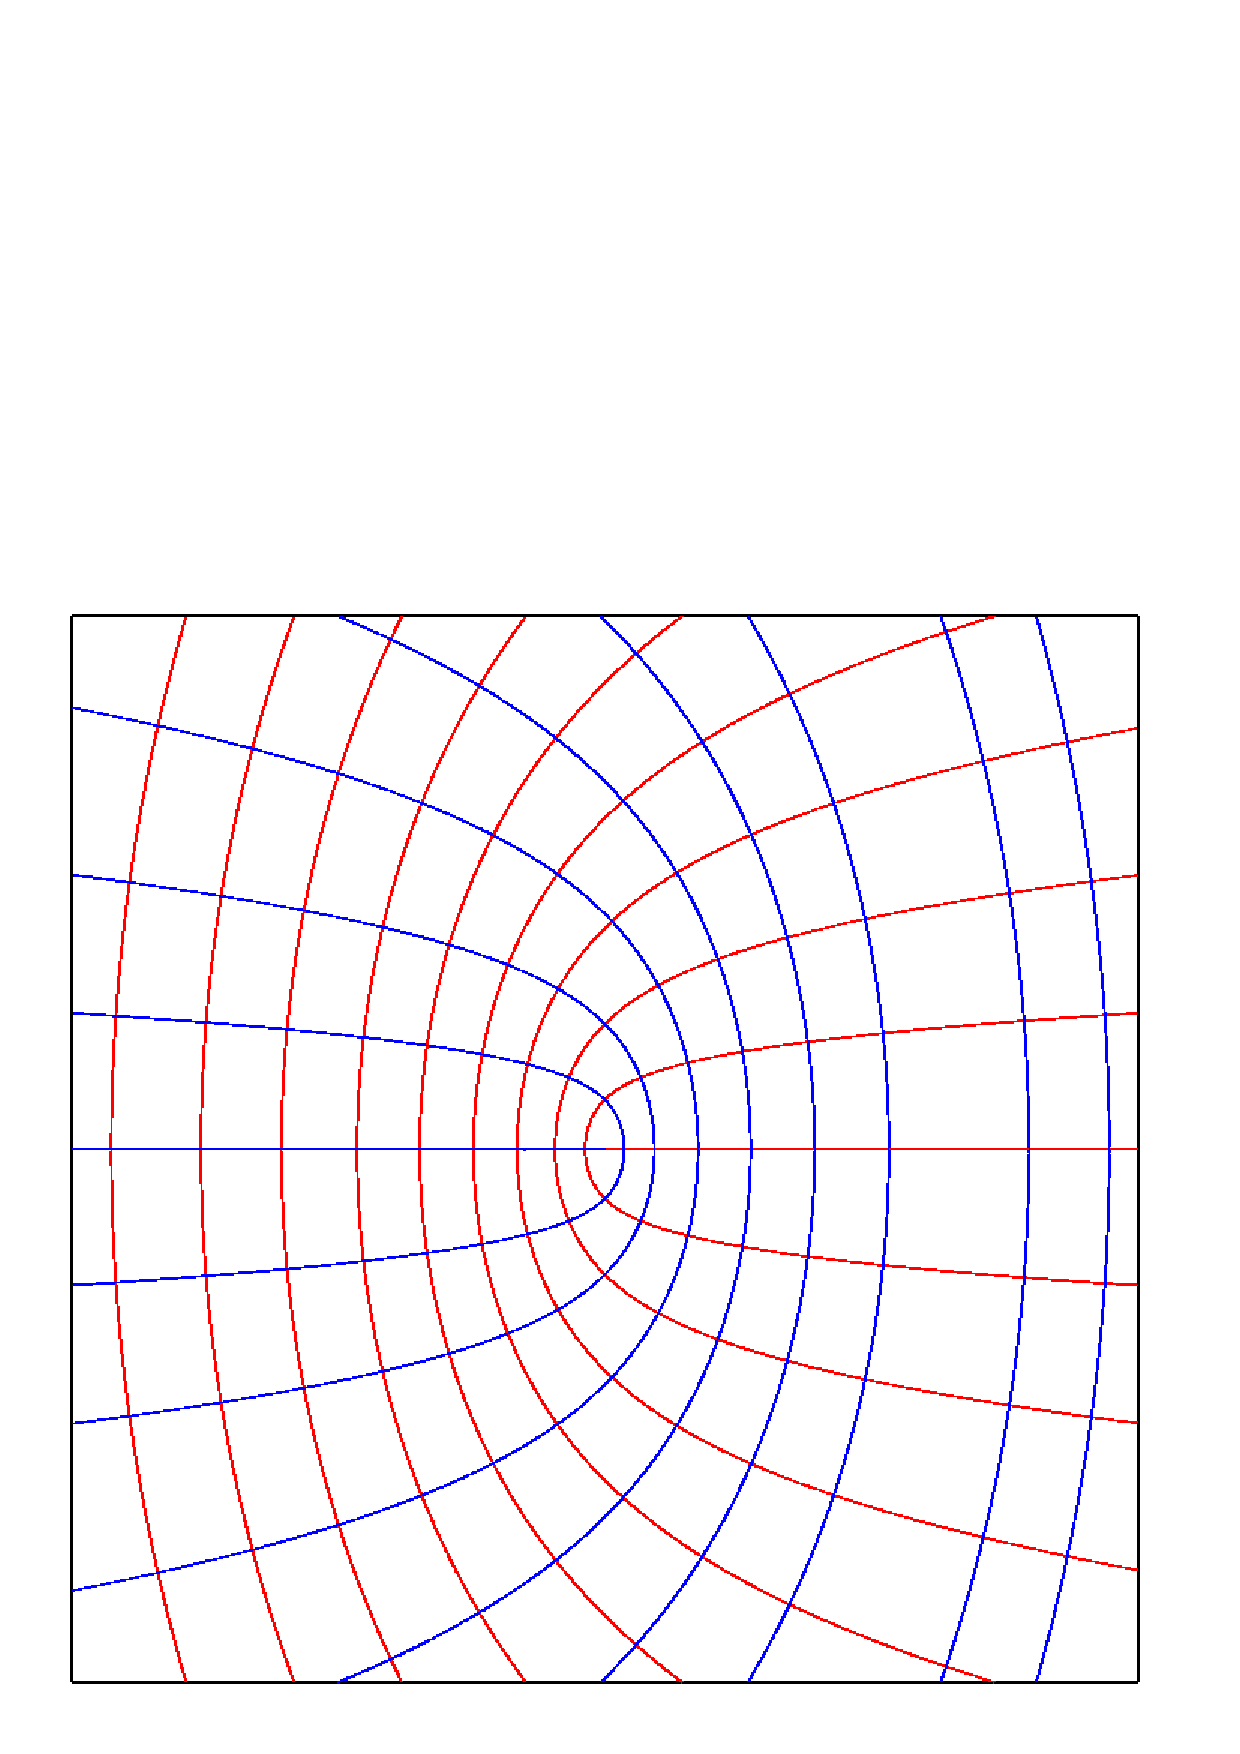
\includegraphics[width=.3\linewidth]{Ridges_3/lemon}
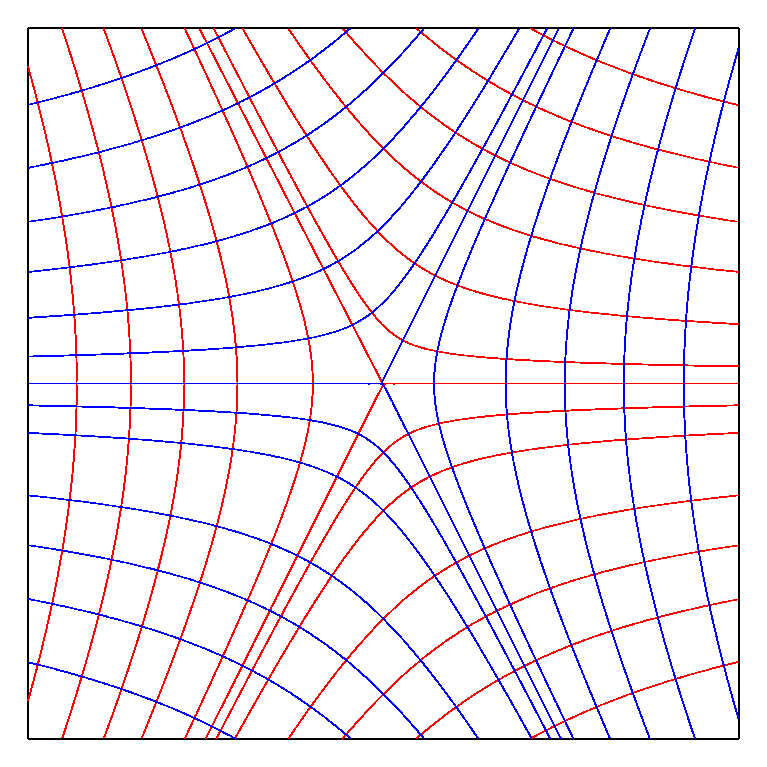
\includegraphics[width=.3\linewidth]{Ridges_3/star}}
\end{ccTexOnly}
\caption{Wedge and trisector umbilics.}
\label{umbilics}
\begin{ccHtmlOnly}
<CENTER> <img border=0 src="./lemon.png" width=200>
 <img border=0 src="./star.png" width=200>
</CENTER>
\end{ccHtmlOnly}
\end{figure}



\section{Extraction of ridges on Triangular Meshes}
%%%%%%%%%%%%%%%%%%%%%%%%%%%%%%%%%
\label{ridge-mesh}

\FC{marching line -> marching triangles???}

\paragraph{Compliant meshes.}
Ridges of a smooth surface are points with prescribed differential
properties, and reporting them from a mesh requires delicate
hypothesis on the geometry of that mesh so as to get a certified
result. In this paragraph, we assume the mesh provided complies with a
number of hypothesis, which guarantee the topology of the ridges
reported matches that of the ridges on the smooth surface. See
\cite{cgal:cp-tdare-05} for a detailed discussion of {\em compliant} meshes.
\medskip

As 0-level set of the extremality coefficients $b_0$ and $b_3$, ridges
are extracted by a marching triangles algorithm \footnote{A marching
triangles algorithm is similar to a marching cubes algorithm, excepted
that a one-manifold is reported.}.
%%
%%on the surface.  
%%
As the signs of these extremality coefficients depends on the
orientation of the principal directions, we expect both extremalities
and vectors orienting the principal direction to be given at each
point vertex of the mesh. Except in the neighborhood of umbilics, if
the mesh is dense enough, a coherent orientation of principal
directions at both endpoints of an edge is chosen such than the angle
between the two vectors is acute. This rule, the {\em acute rule}, is
precisely analyzed in \cite{cgal:tr-cp-tdare-05}.
%%
Moreover, we only seek ridges in triangles such than one can find an
orientation of its three vertices such that the three edges are
coherently oriented by the acute rule. Such triangles are termed
{\em regular}. This said, two remarks are in order.

\FC{above: why do we expect the extremalities to be given since we use
the acute rule???????}

\FC{I introduced the def of a ridge segment type below}

\noindent {\em ---Regular triangles and ridge segments.}
A regular triangle has 0 or 2 edges crossed by a ridge of a given
color (meaning that $b_0$ or $b_3$ change sign on the edge). In the
later case, we say that the triangle contains a ridge segment.
%%
Two methods are provided to compute its type, as elliptic or
hyperbolic. First, if fourth order differential quantities are
provided, one can use the $P_1$ ($P_2$) polynomial of Eq.
(\ref{{eq:taylor_along_line}}) ((\ref{eq:taylor_along_red_line})) for
a blue (red) ridge.
%%
Alternatively, if third order differential quantities only are
available, one may use the geometric method developed in
\cite{cgal:cp-tdare-05}.


Using the notion of ridge segment, a \ccc{Ridge_line} is defined as a
maximal sequence of ridge segments of the same type and connected
together.  Notice the the topology of a \ccc{Ridge_line} is either
that of an interval or a circle.

%We provide two methods to distinguish elliptic and hyperbolic
%ridges. The first one uses the signs of fourth order quantities
%$P_i$. The other uses only third order quantities, details can be
%found in \cite{cgal:cp-tdare-05}.


\FC{above: if fourth order taging used, type = majority of the tags of
the triangle vertices???????}

\noindent {\em ---Non-regular triangles.}  In the neighborhood of umbilics,
triangle are less likely to be regular and the detection of ridges
cannot be relevant by this method.  This is why we propose another
method to detect umbilics independently.


%We provide two methods to distinguish elliptic and hyperbolic
%ridges. The first one uses the signs of fourth order quantities
%$P_i$. The other uses only third order quantities, details can be
%found in \cite{cgal:cp-tdare-05}.


\paragraph{Non compliant meshes.}
%%
For real world applications dealing with coarse meshes, or meshes
featuring degenerate regions or sharp features, meshes conveying some
amount of noise, the hypothesis \cite{cgal:tr-cp-tdare-05} cannot be
met. In that case, it still makes sense to seek loci of points
featuring extremality of estimated principal curvatures, but the
ridges reported may require filtering. For example, if the principal
curvatures are constant ---which is the case on a plane or a cylinder,
then all points are ridge points. In this context, an appealing notion
is that of {\em sharp} ridge or {\em prominent} ridge. Since ridges
are witnessed by zero crossings of $b_0$ and $b_3$, one can expect
erroneous detections as long as these coefficients remain small. In
order to select the most prominent ridge points, we focus on points
where the variation of the curvature is fast along the curvature line.
One can observe that, at a ridge point, according to the equation
\ref{eq:taylor_along_line}, the second derivative of $k_1$ along its
curvature line satisfies $k_1^{''}(0) = P_1/(k_1-k_2)$.  Using this
observation, one can define the {\em sharpness of a ridge} as the
integral of the absolute value of $P_1/(k_1-k_2)$ along the ridge. As
the second derivative of the curvature is homogeneous to the inverse
of the cube of a length, the sharpness is homogeneous to the inverse
of the square of a length. Multiplying the sharpness by the square of
the model size gives a threshold and an associated sharpness-filter
which are scale independent. Another filtering is also available with
the {\em strength } which is the integral of the curvature along the
ridge line
\cite{cgal:yo-ab-hps-04}.





\section{Extraction of Umbilics on Triangular Meshes}
%%%%%%%%%%%%%%%%%%%%%%%%%%%%%%%%%
\label{umbilic-mesh}

%The detection of umbilics is based upon a two stages methods, which
%both require finding a topological disk around the umbilic.
%
%The method combines a minimization and an index computation (of the
%principal direction field) on the neighborhood of each vertex of $T$.

\paragraph{Algorithm.}
Assume each vertex $v$ of the mesh comes with a patch (a topological
disk) around it. Checking whether vertex $v$ is an umbilic is a two
stages process, which are respectively concerned with the variation
of the function $k_1-k_2$ over the patch, and the index of the vertex
computed from the boundary of the patch. More precisely, vertex $v$ is
declared to be an umbilic if the following two conditions are met:
%%
\begin{itemize}
\item
the function $k_1-k_2$ has its minimum at $v$ amongst all the
vertices of the patch;
\item
the deviation $\delta$ of any principal direction along the the patch
boundary, traversed counter-clock-wise (CCW), has prescribed
properties:
%%
\begin{itemize}
\item
$\delta \in ]\pi/2,3\pi/2[$, then the umbilic is called a wedge,
\item
$\delta \in ]-3\pi/2,-\pi/2[$, then the umbilic is called a trisector,
\item
$\delta \geq 3\pi/2$ or $\delta \leq -3\pi/2$ then the umbilic is called non-generic.
\end{itemize}
\end{itemize}

\FC{of any  ppal direction I guess...}

\paragraph{Finding patches around vertices.}
Given a vertex $v$, we aim at defining a collection of triangles
around $v$ so that this collection defines a topological disk on the
triangulation $T$. First we collect the 1-ring triangles. We define
the size $s$ of this 1-ring patch as the (Euclidean) distance from $v$
to its farthest 1-ring vertex neighbor. We then collect recursively
adjacent triangles so that the patch remains a topological disk and
such that these triangles are at distance less than $st$, with $s$ a
user defined parameter. Parameter $t$ is the only parameter of the
algorithm.

\paragraph{Umbilical patches versus ridges.} On a generic surface,
generic umbilics are traversed by one or three ridges. For compliant
meshes, an umbilic can thus be connected to the ridge points located
on the boundary of its patch. This functionality has not been
implemented, and the reader is referred to \cite{cgal:cp-tdare-05} for
more details.

%%%%%%%%%%%%%%%%%%%%%%%
\section{Software Design}
%%%%%%%%%%%%%%%%%%%%%%%
\label{soft}

All classes of this package are templated by the parameter
\ccc{TriangularPolyhedralSurface} which inherits from \ccc{Polyedron_3}
and defines the mesh on which the extraction algorithms are applied.

The differential quantities are provided at vertices of this mesh via
property maps, a concept commonly used in the Boost library. Scalar
data (curvatures and their derivatives) are provided via
\ccc{Vertex2FTPropertyMap} concepts, while  $3d$ vectorial data (principal
directions of curvatures) are provided via
\ccc{Vertex2VectorPropertyMap} concepts. 
The rationale for introducing these concepts is that properties are
used independently from the way they are stored. This enables the user
to store them {\em internally} in extended vertices or {\em externally}
with maps. We provide a class
\ccc{Vertex2Data_Property_Map_with_std_map} to adapt \ccc{std::maps} with 
a \ccc{boost::associative_property_map} to model these concepts.


Output of ridges or umbilics are provided via output iterator.

Extraction of ridges and umbilics are performed by two independent
classes, which we now further describe.

\subsection{Ridge Approximation}
%%%%%%%%%%%%%%%


The main class is
\ccc{Ridge_approximation<TriangularPolyhedralSurface,OutputIt,Vertex2FTPropertyMap,Vertex2VectorPropertyMap>}.
Its construction requires the mesh and the property maps defining the
differential quantities for principal curvatures $k_1$ and $k_2$, the
third order extremalities $b_0$ and $b_3$, the principal directions of
curvature $d_1$ and $d_2$, and the fourth order quantities $P_1$ and
$P_2$ if the tagging of ridges as elliptic or hyperbolic is done using
the polynomials $P_1$ and $P_2$.


Two functions enable to either compute all ridges
\ccc{compute_all_ridges} or only some of them
\ccc{compute_ridges}. 
These functions allows the user to specify how the elliptic/hyperbolic
tagging is carried out.  For the second function, one may further
specify a ridge intersection type, that is an entry in the following
enumeration \ccc{ BLUE_RIDGE, RED_RIDGE, CREST}. 
%%
Notice the rationale for allowing to specify an entry in this enum is
simple: all ridges of such a type can be computed by a single pass
over the triangles of the mesh. This should be clear for the red and
blue ridges. For crests, just notice red and blue crests cannot
intersect over a triangle.
\medskip

\FC{in the interrogation type, why do we have crest .. while it is not
in the enum gathering all types????????}


The ridge lines are stored in
\ccc{Ridge_line} objects and output through an iterator. 
Each ridge line is represented as a list of half-edges of the mesh it
crosses with a scalar defining the barycentric coordinate of the
crossing point with respect to the half-egde endpoints. Each ridge
line comes with its type \ccc{Ridge_type}, its strength and sharpness.

If one chooses to use only third order quantities, the quantities
$P_i$ does not have to be defined. Then the sharpness will not be
defined.

\subsection{Umbilic Approximation}
%%%%%%%%%%%%%%%%%%%%%
The main class is
\ccc{Umbilic_approximation<TriangularPolyhedralSurface,OutputIt,Vertex2FTPropertyMap,Vertex2VectorPropertyMap>}.
Its construction requires the mesh and the property maps defining the
differential quantities for principal curvatures $k_1$ and $k_2$, and
the principal directions of curvature $d_1$ and $d_2$.  The function
\ccc{compute} has a parameter to define the size of the neighborhood of the umbilic.

Umbilics are stored in \ccc{Umbilic} objects, they come with their
type, the vertex of the mesh they are associated to and the list of
half-edges representing the contour of the neighborhood.


\subsection{Models for the property map concepts}
%%%%%%%%%%%%%%%%%%%%%%%%%%%%%%%%%%%%%%%%%%%%%%%%%%%%%%%%%%%%%%%%%%%%%%%%%%%%
The class
\ccc{Vertex2Data_Property_Map_with_std_map<TriangularPolyhedralSurface>}
enables the definition of models for the concepts
\ccc{Vertex2FTPropertyMap}
\ccc{Vertex2VectorPropertyMap} 
using \ccc{std::maps} and \ccc{boost::associative_property_map}.


\section{Examples} 
%%%%%%%%%%%%%%%%%%%%%%%%%%%%%%%%%%%%%%%%%%%%%%%%%%%%%%%%%%%%%%%%%%%%%%%%%%%%
\label{examples}

\FC{provide ranges and default values}

The example program computes ridges and umbilics from an off file. It
uses the Jet fitting package to estimate the differential quantities.
The output file contains data to be visualized with the demo program introspect-qt.
Parameters are 
\begin{itemize}
\item
d, the degree of the jet for the \ccc{Monge_via_jet_fitting} class;
\item
m, the degree of the Monge representation for the \ccc{Monge_via_jet_fitting} class;
\item
a, the number of rings of neighbors collected for the \ccc{Monge_via_jet_fitting} class;
\item
t, the \ccc{Tag_order} for the distinction between elliptic and hyperbolic ridges;
\item
u, the parameter for umbilic patch size.
\end{itemize}

\begin{ccExampleCode} 
#include <CGAL/Ridges.h> 
#include <CGAL/Umbilic.h>

#include <CGAL/Monge_via_jet_fitting.h> 
#include <CGAL/Lapack/Linear_algebra_lapack.h>
 
//this is an enriched Polyhedron with facets' normal
#include "PolyhedralSurf.h"

typedef PolyhedralSurf::Traits          Kernel;
typedef Kernel::FT                      FT;
typedef Kernel::Point_3                 Point_3;
typedef Kernel::Vector_3                Vector_3;

typedef PolyhedralSurf::Vertex          Vertex;
typedef PolyhedralSurf::Vertex_handle   Vertex_handle;
typedef PolyhedralSurf::Vertex_iterator Vertex_iterator;

typedef CGAL::Monge_via_jet_fitting<Kernel>    Monge_via_jet_fitting;
typedef Monge_via_jet_fitting::Monge_form      Monge_form;
typedef Monge_via_jet_fitting::Monge_form_condition_numbers Monge_form_condition_numbers;
      
typedef CGAL::Vertex2Data_Property_Map_with_std_map<PolyhedralSurf> Vertex2Data_Property_Map_with_std_map;
typedef Vertex2Data_Property_Map_with_std_map::Vertex2FT_map Vertex2FT_map;
typedef Vertex2Data_Property_Map_with_std_map::Vertex2Vector_map Vertex2Vector_map;
typedef Vertex2Data_Property_Map_with_std_map::Vertex2FT_property_map Vertex2FT_property_map;
typedef Vertex2Data_Property_Map_with_std_map::Vertex2Vector_property_map Vertex2Vector_property_map;

//RIDGES
typedef CGAL::Ridge_line<PolyhedralSurf> Ridge_line;
typedef CGAL::Ridge_approximation < PolyhedralSurf,
				    back_insert_iterator< std::vector<Ridge_line*> >,
				    Vertex2FT_property_map,
				    Vertex2Vector_property_map > Ridge_approximation;
  

//UMBILICS
typedef CGAL::Umbilic<PolyhedralSurf> Umbilic;
typedef CGAL::Umbilic_approximation < PolyhedralSurf,
				      back_insert_iterator< std::vector<Umbilic*> >, 
				      Vertex2FT_property_map, 
				      Vertex2Vector_property_map > Umbilic_approximation;

//create property maps
Vertex2FT_map vertex2k1_map, vertex2k2_map, 
  vertex2b0_map, vertex2b3_map, 
  vertex2P1_map, vertex2P2_map;
Vertex2Vector_map vertex2d1_map, vertex2d2_map;

Vertex2FT_property_map vertex2k1_pm(vertex2k1_map), vertex2k2_pm(vertex2k2_map), 
  vertex2b0_pm(vertex2b0_map), vertex2b3_pm(vertex2b3_map), 
  vertex2P1_pm(vertex2P1_map), vertex2P2_pm(vertex2P2_map);
Vertex2Vector_property_map vertex2d1_pm(vertex2d1_map), vertex2d2_pm(vertex2d2_map);

int main(int argc, char *argv[])
{  
  //compute differential quantities with the jet fitting package
	...
  //initialize the property maps
	...
   //---------------------------------------------------------------------------
  //Ridges
  //--------------------------------------------------------------------------
  Ridge_approximation ridge_approximation(P, 
					  vertex2k1_pm, vertex2k2_pm,
					  vertex2b0_pm, vertex2b3_pm,
					  vertex2P1_pm, vertex2P2_pm,
					  vertex2d1_pm, vertex2d2_pm);
  std::vector<Ridge_line*> ridge_lines;
  back_insert_iterator<std::vector<Ridge_line*> > ii(ridge_lines);
  
  //Find BLUE_RIDGE, RED_RIDGE, CREST_RIDGE
     ridge_approximation.compute_ridges(CGAL::BLUE_RIDGE, ii, tag_order);  
     ridge_approximation.compute_ridges(CGAL::RED_RIDGE, ii, tag_order);  
     ridge_approximation.compute_ridges(CGAL::CREST_RIDGE, ii, tag_order);  
  // or do it at once
  // ridge_approximation.compute_all_ridges(ii, tag_order);  
 
  std::vector<Ridge_line*>::iterator iter_lines = ridge_lines.begin(), 
    iter_end = ridge_lines.end();
  //OpenGL output
  for (;iter_lines!=iter_end;iter_lines++) (*iter_lines)->dump_4ogl(out_4ogl);
    
  //verbose txt output 
  if (verbose) 
    for (iter_lines = ridge_lines.begin();iter_lines!=iter_end;iter_lines++) 
      out_verb << **iter_lines; 

  //---------------------------------------------------------------------------
  // UMBILICS
  //--------------------------------------------------------------------------
  Umbilic_approximation umbilic_approximation(P, 
					      vertex2k1_pm, vertex2k2_pm,
					      vertex2d1_pm, vertex2d2_pm);
  std::vector<Umbilic*> umbilics;
  back_insert_iterator<std::vector<Umbilic*> > umb_it(umbilics);
  umbilic_approximation.compute(umb_it, umb_size);

  std::vector<Umbilic*>::iterator iter_umb = umbilics.begin(), 
    iter_umb_end = umbilics.end();
  // output
  std::cout << "nb of umbilics " << umbilics.size() << std::endl;
  for (;iter_umb!=iter_umb_end;iter_umb++) std::cout << **iter_umb;
}
\end{ccExampleCode}

For figure \ref{ellipsoid_ridges_example}, the data are computed with
the call
\begin{ccExampleCode}
./blind -f data/ellipsoid_u_0.02.off -d4 -m4 -a3 -t3
\end{ccExampleCode}
and the visualization with 
\begin{ccExampleCode}
 ../../demo/Ridges_3/introspect-qt data/ellipsoid_u_0.02.off data/data_ellipsoid_u_0.02.offRIDGES-d4-m4-t4-a3-p0.4ogl.txt 0 0
\end{ccExampleCode}
In addition, the four wedge umbilics are detected, the standart output is 
\begin{ccExampleCode}
nb of umbilics 4
Umbilic at location (-0.80899 0.00426003 0.293896) of type wedge
Umbilic at location (-0.811197 0.0122098 -0.292259) of type wedge
Umbilic at location (0.808372 -0.00551307 -0.29431) of type wedge
Umbilic at location (0.81413 0.0018689 0.290339) of type wedge
\end{ccExampleCode}


\begin{figure}[!ht]
\begin{ccTexOnly}
\centerline{
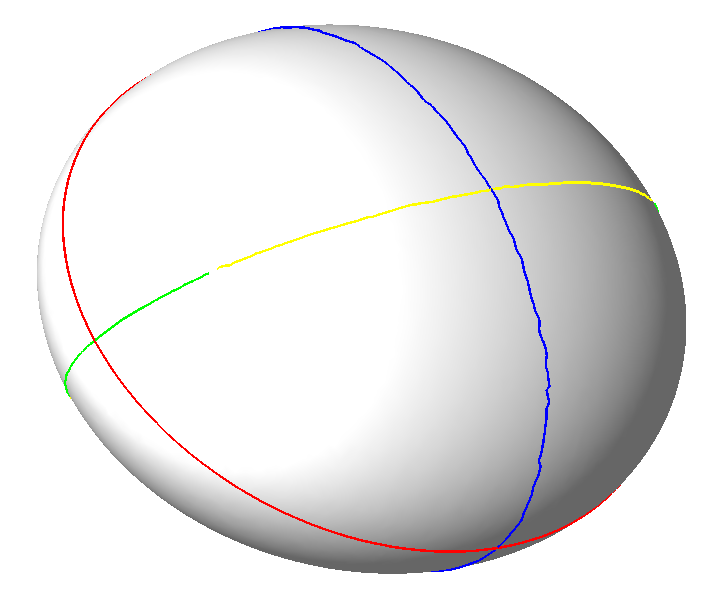
\includegraphics[width=.5\linewidth]{Ridges_3/ellipsoid_ridges}}
\end{ccTexOnly}
\caption{Ridges on the ellipsoid, normals pointing outward.
 Color coding~: \ccc{BLUE_ELLIPTIC_RIDGE} are blue,
\ccc{BLUE_HYPERBOLIC_RIDGE} are green, \ccc{RED_ELLIPTIC_RIDGE} are red and 
\ccc{RED_HYPERBOLIC_RIDGE} are yellow. }
\label{ellipsoid_ridges_example}
\begin{ccHtmlOnly}
<CENTER> <img border=0 src="./ellipsoid_ridges.png" width=400>
</CENTER>
\end{ccHtmlOnly}
\end{figure}


Figures \ref{fig:mechanical_crest_filtered-intro}, illustrates the
filtering of crest ridges on a mechanical part. Data are computed with 
\begin{ccExampleCode}
./blind -f data/mecanic.off -d4 -m4 -a4 -t4
\end{ccExampleCode}
The last parameters of the visualization program of the demo are
threshold for the strength and the sharpness. This enables the three
different images to be produced with the same data.

\begin{figure}[htb] 
\begin{ccTexOnly}
\centerline{ 
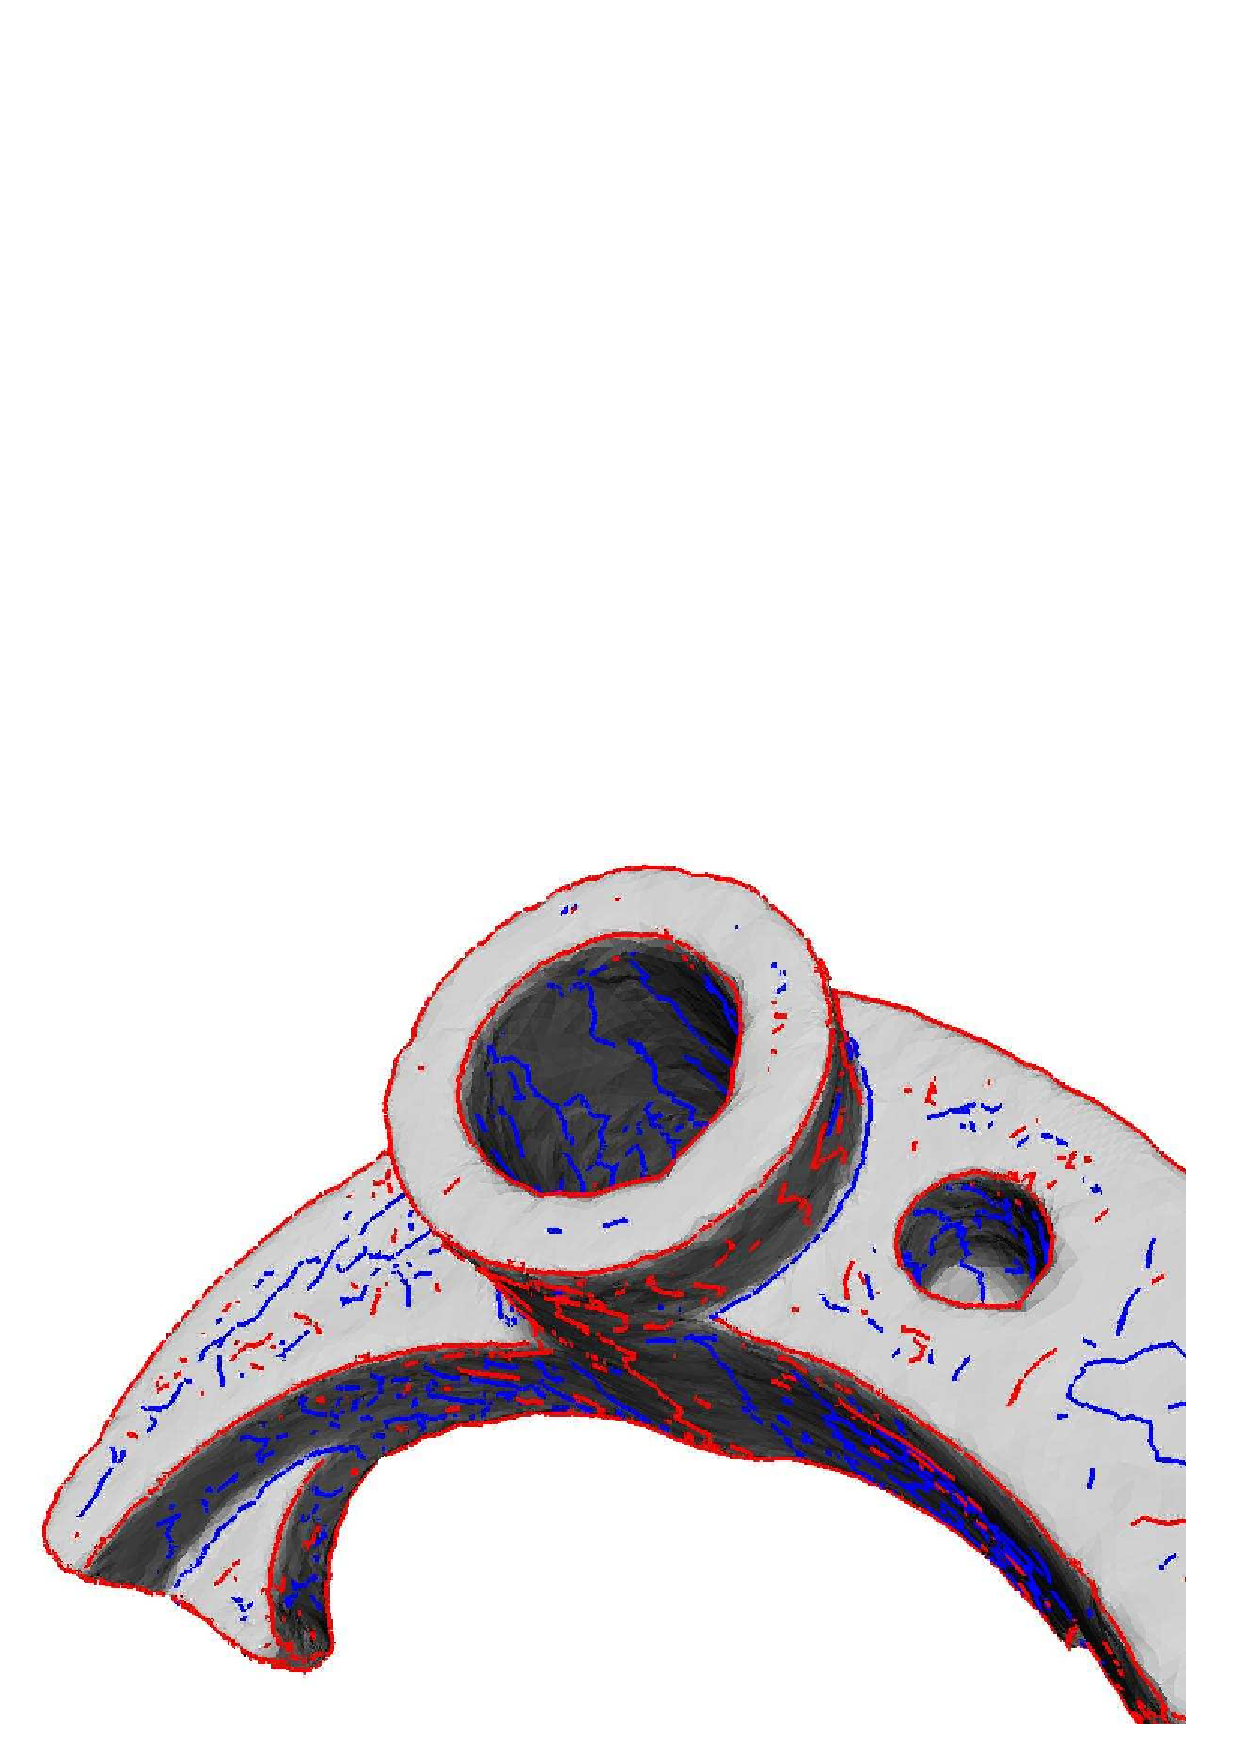
\includegraphics[width=.45\linewidth]{Ridges_3/mecanic-sub1_crest-jpg}
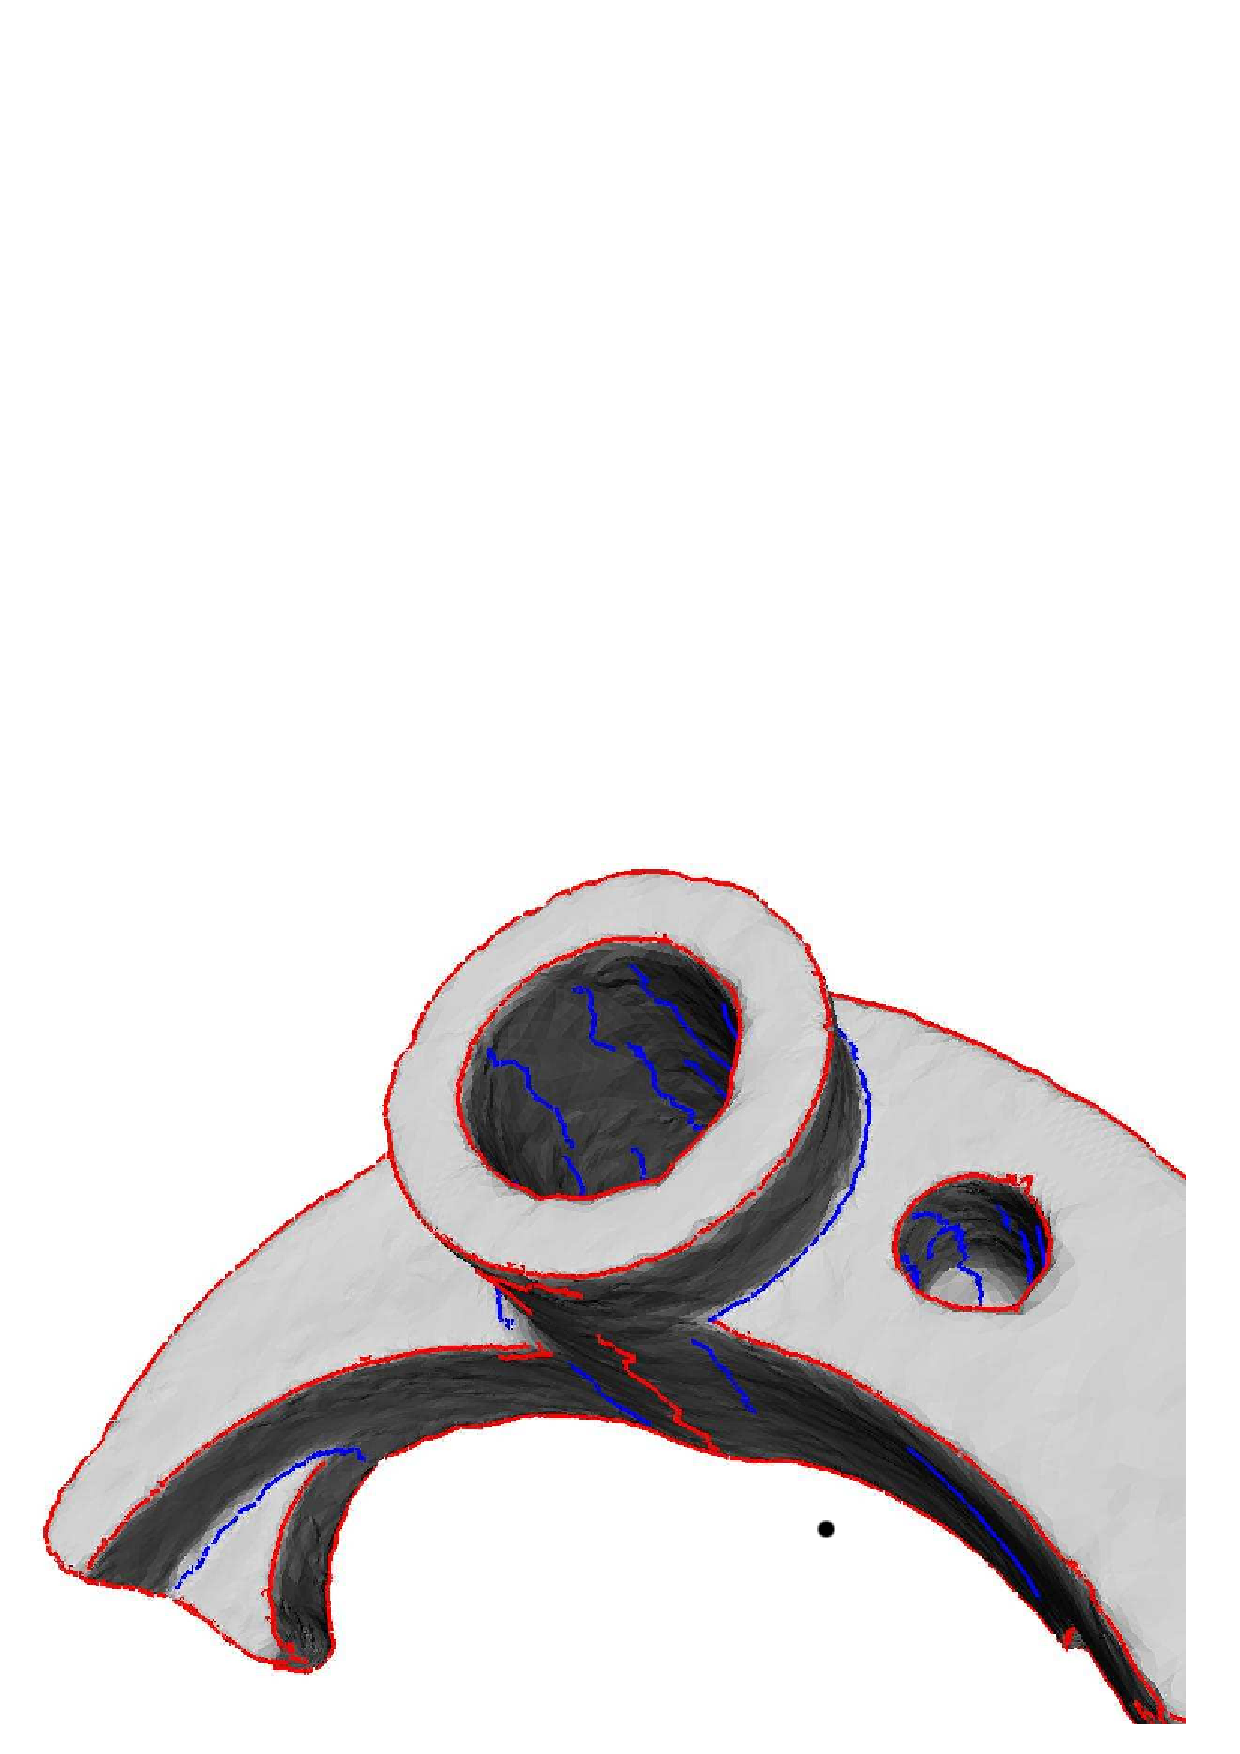
\includegraphics[width=.45\linewidth]{Ridges_3/mecanic-sub1_crestTweight1-jpg}}
\centerline{
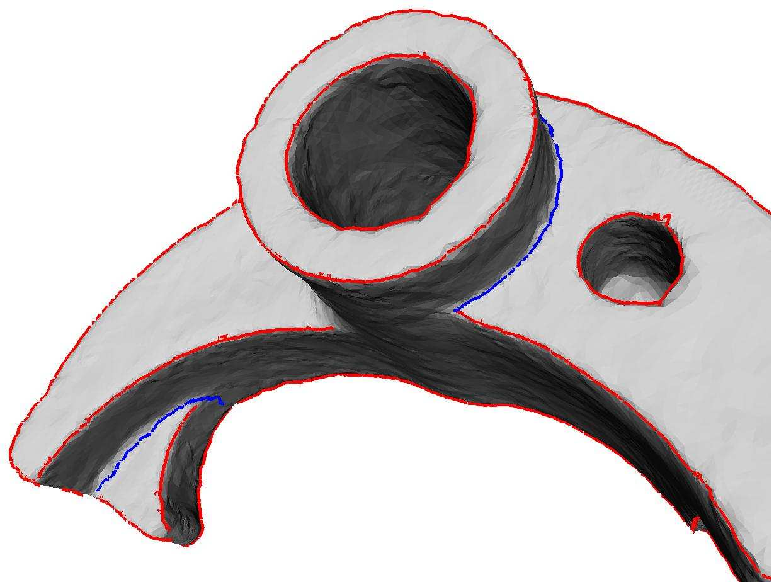
\includegraphics[width=.6\linewidth]{Ridges_3/mecanic-sub1_crestTweight1Tsharp7-jpg}}
\end{ccTexOnly}
\caption{Mechanical part (37k pts): (a) All crest lines, (b) crests filtered
with the strength threshold 1 and (c) crests filtered with the sharpness threshold 100 000.
%%
Notice that any point on a flat or cylindrical part lies on two
ridges, so that the noise observed on the top two Figs. is
unavoidable. It is however easily filtered out with the sharpness on
the bottom figure.}
\label{fig:mechanical_crest_filtered-intro} 
\begin{ccHtmlOnly}
<CENTER> <img border=0 src="./mecanic-sub1_crest-jpg.png" width=200>
 <img border=0 src="./mecanic-sub1_crestTweight1-jpg.png" width=200>
</CENTER>
<CENTER>
 <img border=0 src="./mecanic-sub1_crestTweight1Tsharp7-jpg.png" width=400>
</CENTER>
\end{ccHtmlOnly}
\end{figure} 
